% Shared standalone design for the editable figure reconstructions.
\documentclass[tikz,border=5pt,10pt]{standalone}
\usepackage[T1]{fontenc}
\usepackage[utf8]{inputenc}
\usepackage{newpxtext,newpxmath}
\usepackage[scaled=.94]{sourcesanspro}
\usepackage{pgfplots}
\pgfplotsset{compat=1.18}
\usetikzlibrary{arrows.meta,calc,positioning,decorations.pathreplacing,
  decorations.markings,patterns,matrix,shapes.geometric,fit,backgrounds,
  intersections,angles,quotes}
\definecolor{ink}{HTML}{203746}
\definecolor{accent}{HTML}{146C78}
\definecolor{muted}{HTML}{667780}
\definecolor{signalred}{HTML}{B94B44}
\color{ink}
\tikzset{>=Latex,line width=.8pt,
  every node/.style={font=\small},
  axis/.style={->,draw=muted,line width=.5pt},
  guide/.style={draw=muted,dashed,line width=.45pt},
  curve/.style={draw=accent,line width=1pt},
  marker/.style={circle,fill=accent,inner sep=1.5pt},
  labelbox/.style={fill=white,inner sep=2pt}}

\begin{document}
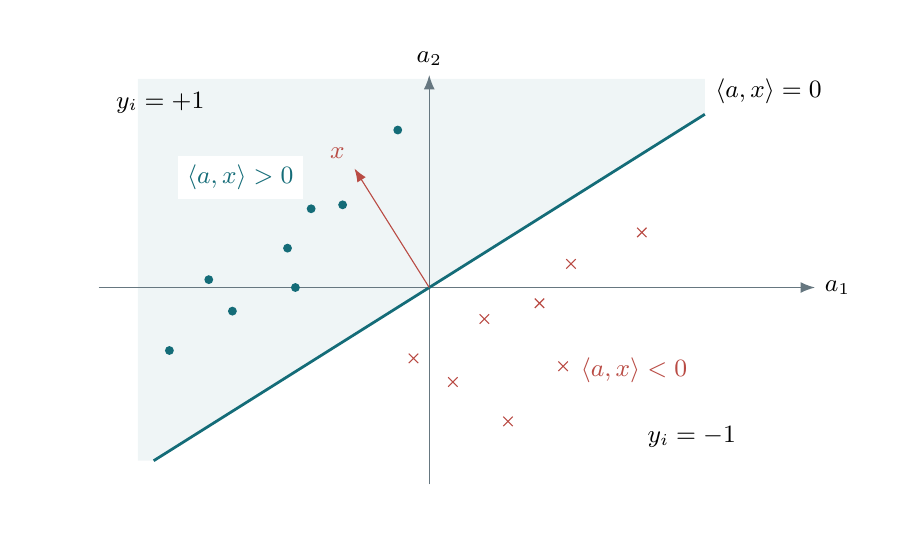
\begin{tikzpicture}
\path[use as bounding box] (-.6,-.6) rectangle (10.3,5.8);

\fill[accent!7] (1,.3)--(8,4.7)--(8,5.15)--(.8,5.15)--(.8,.3)--cycle;
\draw[axis] (.3,2.5)--(9.4,2.5) node[right] {$a_1$};\draw[axis] (4.5,0)--(4.5,5.2) node[above] {$a_2$};
\draw[curve] (1,.3)--(8,4.7) node[above right] {$\langle a,x\rangle=0$};
\draw[->,signalred] (4.5,2.5)--(3.55,4.011364) node[above left] {$x$};
\node[anchor=west] at (.4,4.85) {$y_i=+1$};\node[anchor=west] at (7.15,.6) {$y_i=-1$};
\node[accent,fill=white] at (2.1,3.9) {$\langle a,x\rangle>0$};
\node[signalred,fill=white] at (7.1,1.45) {$\langle a,x\rangle<0$};
\fill[accent] (1.7,2.6) circle (1.6pt);
\fill[accent] (2,2.2) circle (1.6pt);
\fill[accent] (2.7,3) circle (1.6pt);
\fill[accent] (2.8,2.5) circle (1.6pt);
\fill[accent] (3.4,3.55) circle (1.6pt);
\fill[accent] (3,3.5) circle (1.6pt);
\fill[accent] (1.2,1.7) circle (1.6pt);
\fill[accent] (4.1,4.5) circle (1.6pt);
\draw[signalred] (4.24,1.54)--(4.359999999999999,1.6600000000000001) (4.24,1.6600000000000001)--(4.359999999999999,1.54);
\draw[signalred] (4.74,1.24)--(4.859999999999999,1.36) (4.74,1.36)--(4.859999999999999,1.24);
\draw[signalred] (5.140000000000001,2.04)--(5.26,2.16) (5.140000000000001,2.16)--(5.26,2.04);
\draw[signalred] (5.840000000000001,2.2399999999999998)--(5.96,2.36) (5.840000000000001,2.36)--(5.96,2.2399999999999998);
\draw[signalred] (6.140000000000001,1.44)--(6.26,1.56) (6.140000000000001,1.56)--(6.26,1.44);
\draw[signalred] (6.24,2.7399999999999998)--(6.359999999999999,2.86) (6.24,2.86)--(6.359999999999999,2.7399999999999998);
\draw[signalred] (7.140000000000001,3.14)--(7.26,3.2600000000000002) (7.140000000000001,3.2600000000000002)--(7.26,3.14);
\draw[signalred] (5.44,0.74)--(5.56,0.8600000000000001) (5.44,0.8600000000000001)--(5.56,0.74);
\end{tikzpicture}
\end{document}
